\section{Responsabilités du sous-système} % 1.1
Le sous-système de communication est responsable des fonctions suivantes :

\renewcommand{\labelitemi}{$\bullet$}
\begin{itemize}
    \item \textbf{Transmission des données de charge utile} vers le sol, en fonction des exigences de la mission.
    \item \textbf{Adaptabilité à la mission}, offrant une large gamme de débits de données, de bandes passantes et de niveaux de criticité.
    \item \textbf{Envoi des données du vaisseau spatial} vers le sol pour les opérations, notamment :
    \begin{itemize}
    		
        \item \textbf{Données d’attitude et d’accélération} : issues de capteurs solaires, capteurs stellaires, gyroscopes, accéléromètres, etc.
        \item \textbf{Données de maintenance} : incluant les températures, pressions, tensions, courants, etc.
    \end{itemize}
    
    \item \textbf{Réception des commandes} transmises depuis le sol pour le pilotage et l'exploitation du vaisseau spatial.
\end{itemize}

\begin{figure}[H] % H force l'affichage ici
    \centering
    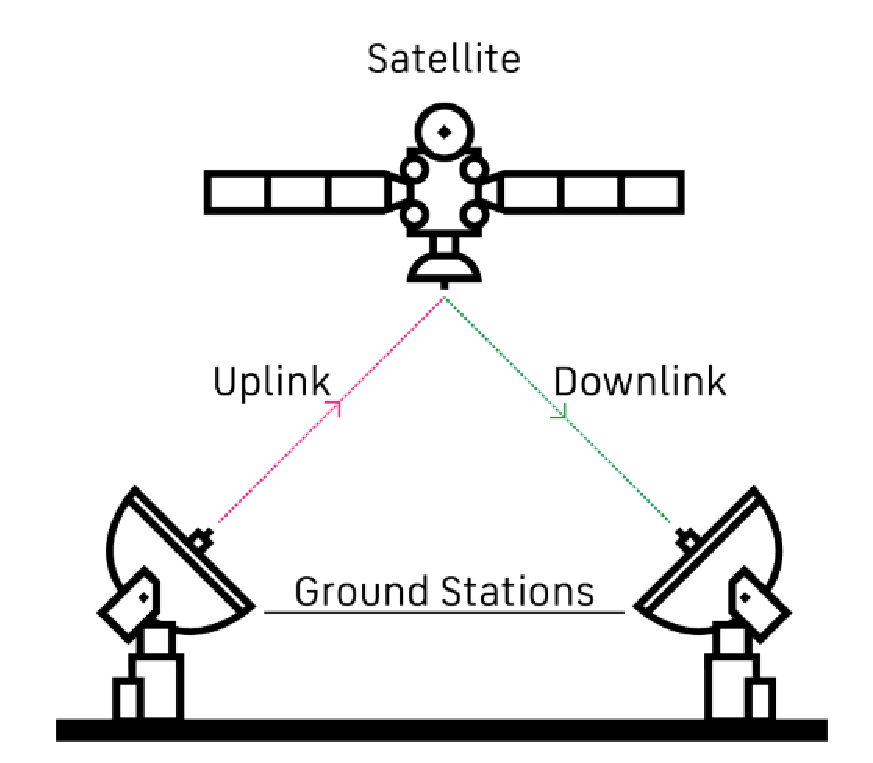
\includegraphics[width=0.5\textwidth]{figures/6-120.eps}
    
    \caption{Un scénario de communication par satellite de base. Le satellite relaie les signaux reçus vers les segments terrestres situés dans son empreinte. Image d'Inmarsat}
    \label{fig:communication2}
\end{figure}



\begin{itemize}
    \item Définition d'une architecture de communication, qui comprend le bus spatial et les segments terrestres.
    \begin{itemize}
        \item Sélection d'une fréquence radio et obtention de la licence pour cette radiofréquence.
        \item Jongler avec le nombre et la position des stations terrestres disponibles
    \end{itemize}
    \item Sélection et codage de la compression, de l'encodage et de la modulation des signaux pour équilibrer la perte et la bande passante.
    \item Sélectionnez une technologie de communication qui respecte les contraintes de masse, de volume, de puissance et les réglementations et qui répond aux exigences de la mission
    \item Vérification de la fermeture du budget de liaison de communication en fonction des technologies sélectionnées et de l'architecture de la station au sol   
\end{itemize}





